\chapter{Theoretical background}
%Here you identify and give the theoretical background needed in this report, with proper references to each literature reference used. The selection of what to include should be discussed and agreed with the supervisors. Theory may involve concepts, definitions, methods, regulations/key standards, theory to explain specific system behavior, and so on.
In this chapter we are going to investigate some of the key concepts related to pattern recognition and shape detection in imagery. 

\section{Shape detection}
Identifying geometric shapes in computer vision has been a classical problem for decades. There are many theories related to what is the best way of detecting a particular shape in an image, with shapes defines as two dimensional features of an object that are invariant to scene factors, or whose variation can be modeled easily \citep{Moon2002}.

\subsection{The standard approach}
Most images are based on a raster format, meaning that pixels in the image are structured as an array or grid, where each pixel is associated with a position (row and column), and a numeric value. Raster images can represent a range of different shapes, where a point can be represented by a single pixel and a circle by a contiguous collection of pixels \citep{Worboys2003}. Even though rasters are easy to work with in most computer systems, since they are represented the way that they are, they do not contain any information about the topology of the objects in the image. For example, there is no way of knowing if a pixel is contained within a certain object or not. In order to identify objects, one approach is therefore to detect edge pixels.

There are many well-known methods that are used in order to find an objects external contour, such as the generalized Hough transform (GHT) \citep{Ballard1981}, fitting of polynomial curves and applying band matching after edge detection.

In recent years shape detection algorithms have come to increasingly rely on superpixel algorithms, which groups pixels into perceptually meaningful atomic regions \citep{Achanta2012}. Such regions replace the regular, rigid structure of the raster grid, as shown in \autoref{fig:superpixels}.

\begin{figure}[!h]
	\centering
	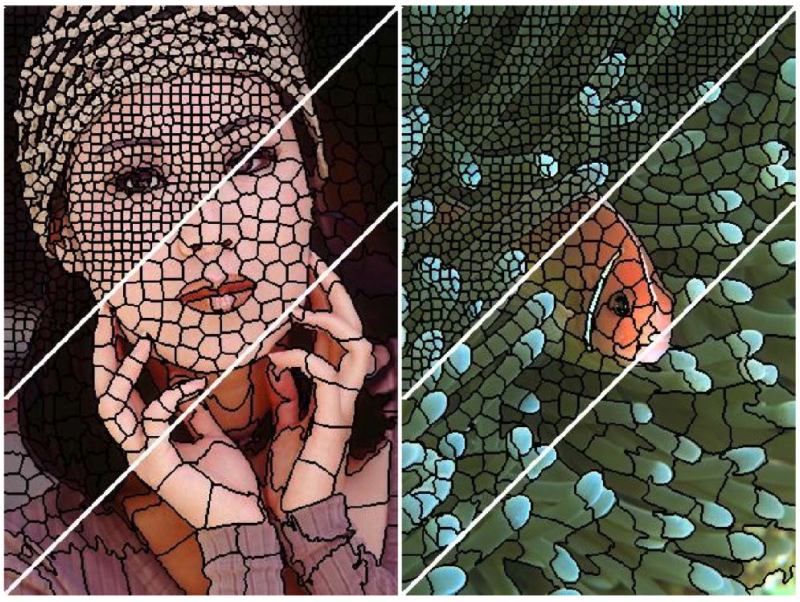
\includegraphics[scale=0.3]{fig/superpixels}
	\caption{Visualization of image segmentation using SLIC \citep{Achanta2012}}
	\label{fig:superpixels}
\end{figure}

When constructing superpixels, there are some properties of the algorithm that are desirable, regardless of the problem that are being solved. These are, according to \citep{Achanta2012}, the following three points:

\begin{itemize}
	\item Superpixels should adhere well to image boundaries
	\item When used to reduce computional complexity as a preprocessing step, superpixels should be fast to compute, memory efficient, and simple to use.
	\item When used for segmentation purposes, superpixels should both increase the speed and improve the quality of the results.
\end{itemize}

\cite{Achanta2012} proposes a superpixel-segmentation algorithm (SLIC), which in their opinion is best suited to meet these demands. They compare their algorithm to a variety of state-of-the-art superpixel methods, and conclude that none of the existing methods are satisfactory in regards to the points.

\subsubsection*{Simple Linear Iterative Clustering (SLIC)}
The SLIC algorithm is fairly simple to understand. One of its key principles is that, by limiting the search space for each cluster center (points in the regular raster grid), it reduces the search speed significantly. This is achievable due to the fact that one of the primary goals of algorithm is to create a set of approximately equal sized superpixels. Thus, instead of searching the whole raster grid for each cluster center, the algorithm only has to search for edge pixels at a distance equal to D, as shown in \autoref{eq:distanceSuperpixel}.

\begin{equation}
	D'=\sqrt{\left(\frac{d_{c}}{m}\right)^{2} + \left(\frac{d_{s}}{S}\right)^{2}}
	\label{eq:distanceSuperpixel}
\end{equation}

In \autoref{eq:distanceSuperpixel} $d_{c}$ is the euclidean distance between two pixels in terms of color and $d_{s}$ is the pixels euclidean, spatial distance. Furthermore, $S$ is the sampling interval of the cluster centers ($S = \sqrt{N/k}$, where N is the number of pixels in the grid and k is the desired number of superpixels) and $m$ is a fixed constant based on the color diversity in the image.

Since the algorithm generates superpixels by clustering pixels based on their color and spatial proximity, creating a 5 dimensional, \textit{labxy} space, one would think that the distance could be found by simply taking the 5D euclidean distance. However, it turns out that for large superpixels, spatial distance outweigh the color proximity. Which is why the two distances $d_{c}$ and $d_{s}$ are weighted.

\subsection{The cognitive approach}

Links:

https://www.pyimagesearch.com/2014/10/20/finding-shapes-images-using-python-opencv/\\
https://www.pyimagesearch.com/2016/02/08/opencv-shape-detection/
\\
http://melvincabatuan.github.io/SLIC-Superpixels/
\\
